\documentclass[UTF8]{article}
% 中文支持
\usepackage[UTF8]{ctex}	
% pdf调用 封面
\usepackage{pdfpages}
% color宏包
\usepackage{color}  
% 导入图片
\usepackage{caption}
\usepackage{graphicx, subfig}
% 防止图片乱跑
\usepackage{float}
% 支持数学符号
\usepackage{amsmath}
% 支持代码块
\usepackage{listings}
% pdf加入大纲
\usepackage{hyperref}
% 大纲去红框
\hypersetup{hidelinks,
	colorlinks=true,
	allcolors=black,
	pdfstartview=Fit,
	breaklinks=true
}
% 消除警告
\usepackage{lmodern}

% 设置页面的环境,a4纸张大小,左右上下边距信息
\usepackage[a4paper, left=31.8mm, right=31.8mm, top=25.4mm, bottom=25.4mm]{geometry}

% 代码块的基本设置
\lstset{
 columns=fixed,       
 numbers=left,                                        % 在左侧显示行号
 numberstyle=\tiny\color{gray},                       % 设定行号格式
 frame=none,                                          % 不显示背景边框
 backgroundcolor=\color[RGB]{245,245,244},            % 设定背景颜色
 keywordstyle=\color[RGB]{40,40,255},                 % 设定关键字颜色
 numberstyle=\footnotesize\color{darkgray},           
 commentstyle=\it\color[RGB]{0,96,96},                % 设置代码注释的格式
 stringstyle=\rmfamily\slshape\color[RGB]{128,0,0},   % 设置字符串格式
 showstringspaces=false,                              % 不显示字符串中的空格
 language=matlab,                                        % 设置语言
}

% 生成目录
% \tableofcontents
% \cleardoublepage

% 导入图片
% \begin{figure}[H]
%     \centering % 居中 
%     % 图片文件的相对路径
%     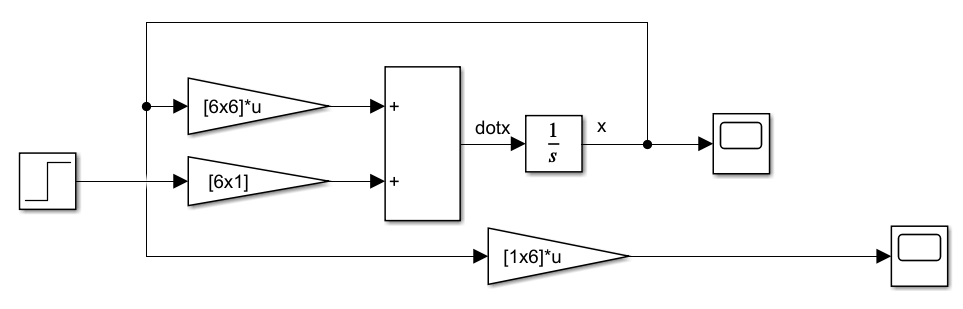
\includegraphics[width=.8\textwidth]{figure/exp1_1_model.png} 
%     \caption{Simulink模型} % caption是图片的标题
%     % \label{img} % 此处的label相当于一个图片的专属标志,目的是方便上下文的引用
% \end{figure}

% 导入代码
% \begin{lstlisting}
% a
% \end{lstlisting}


% 《PLC 与 DCS 综合设计》预习报告
\begin{document}

\begin{titlepage}
% 封面信息

\includepdf[pages={1}]{cover.pdf}
\end{titlepage}

%
\section{我所了解的PLC与DCS}
% 文字 1000 字内,用自己的话去说明什么是 PLC 与 DCS?有何不同(各自特点)?未来发展趋势?)要求:语句通顺,格式规范,层次逻辑清晰。

\paragraph{什么是 PLC 与 DCS?}~{}

PLC即Programmable Logic Controller,又称可编程逻辑控制器,是工业自动化领域中一种重要的控制系统。在工业领域中,PLC主要用于实现工业生产过程的自动化控制。它是一种专门用于对各种输入信号进行逻辑运算、顺序控制和定时控制的设备。PLC具有可靠性高、抗干扰能力强、易于编程和维护等特点。它通常用于开关量控制,如电机启停、阀门开关等。此外,PLC可以通过梯形图、指令表等形式的编程语言进行编程,实现对特定工业过程的精确控制。

DCS即Distributed Control System,又称分布式控制系统,是一种用于实现大型工业过程集中监控和控制的系统。它由多个分散的控制单元组成,并且通过计算机通信网络连接在一起,实现对整个生产过程的集中监控和控制。DCS具有高度的集成性、灵活性和可扩展性,可以用于对不同规模和复杂度的工业过程进行控制。DCS通常用于模拟量和连续量的控制,如温度、压力、流量等参数的监测和调节。

\paragraph{各自的特点和不同之处}~{}
\\
从特点上来看,PLC和DCS有以下不同之处:
\begin{itemize}
    \item 功能定位:PLC主要用于开关量控制,而DCS主要用于模拟量控制;
    \item 结构形式:PLC通常是单个设备,而DCS是由多个分散的控制单元组成的系统;
    \item 通信方式:PLC通常采用点对点通信,而DCS采用总线或网络通信;
    \item 可编程性:PLC具有较高的可编程性,可以根据需要灵活编写程序;而DCS的可编程性相对较低,主要通过硬件配置来实现控制功能;
    \item 应用范围:PLC适用于小型、简单的工业过程控制,而DCS适用于大型、复杂的工业过程监控和控制。
\end{itemize}

\paragraph{未来的发展趋势}~{}

PLC和DCS作为工业自动化领域中两种非常重要的控制系统,目前它们在功能、结构和应用领域上都存在着一定的差异。随着工业自动化技术的不断发展,两者都将面临一些新的挑战和机遇。一方面,PLC将更加注重智能化和网络化的发展,提高数据处理和分析能力,实现更高效的生产控制。另一方面,DCS将更加注重系统集成和跨平台的应用,为工业生产问题提供更全面的解决方案。总的来说,PLC和DCS都将朝着智能化、网络化和集成化的方向发展,以适应不断变化的工业需求。

\section{编程,完成$f(x) = ax^2 + bx + c,\ f(x) = 0$的解}
% 要求:
% 要求 1. a、b、c 为任意输入的实数,按“启动”按钮,给出求解的复数范围内解(实部与虚部分开展示)。 需要判断 a = 0,a =b=0、c≠ 0 等各种情况;
% 要求 2. 依据解的情况,采用 1 个指示灯说明:1 个解(点亮),2 个解(1 秒闪烁,含相同解),无解(输入错误)等情况(0.5 秒闪烁);复数解具体值需要正确显示(无解置 0)。
% 要求 3. 给出程序细节(抄袭 0 分)
% 报告:独立完成,11 月 15 号班级负责人交到信息楼 102,过期不候。

%%
\subsection{变量设置}
如下图所示,本程序在默认变量表中设置所需参数。$Real$类型变量“变量1(a)”、“变量2(b)”和“变量3(c)”分别表示一元二次方程$ax^2 + bx + c = 0$中的系数$a,\ b,\ c$;$Bool$类型变量“指示灯”用于设置HMI界面中指示灯的亮灭状态;变量$con1,\ con2,\ con3$用于设置指示灯不同的亮灭状态(常亮、以1s为周期闪烁、以0.5s为周期闪烁);变量“$delta$”为中间变量,用于判断一元二次方程解的情况(两个实数解、共轭复数解);此外,设置了变量“$x1$”,“$x2$”,“实部”和“虚部”用于表示对应情况下方程解的具体值:
\begin{figure}[H]
    \centering % 居中 
    % 图片文件的相对路径
    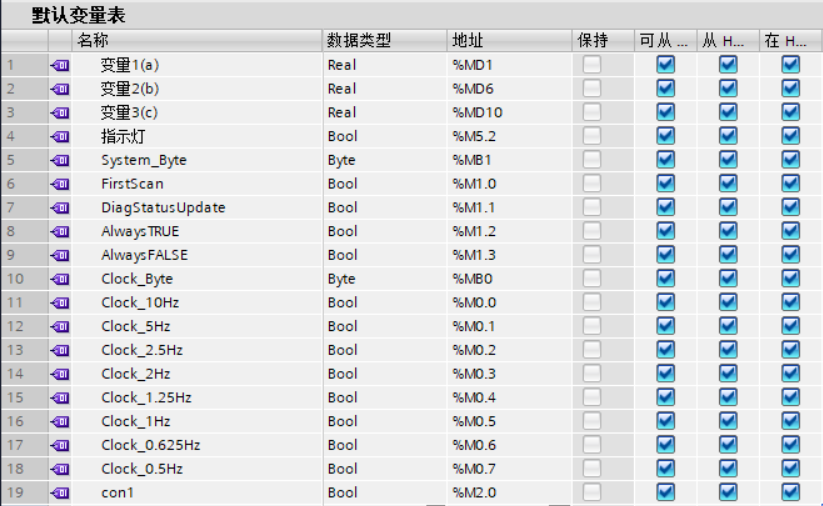
\includegraphics[width=.8\textwidth]{figure/默认变量表1.png} 
    \caption{默认变量表} % caption是图片的标题
    % \label{img} % 此处的label相当于一个图片的专属标志,目的是方便上下文的引用
\end{figure}
\begin{figure}[H]
    \centering % 居中 
    % 图片文件的相对路径
    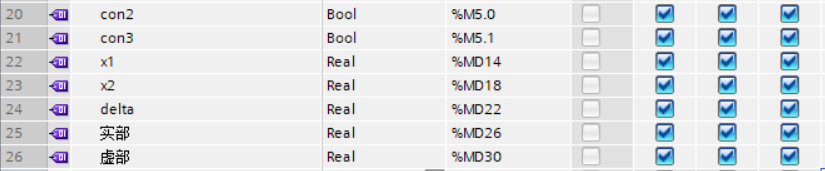
\includegraphics[width=.8\textwidth]{figure/默认变量表2.png} 
    \caption{默认变量表(续)} % caption是图片的标题
    % \label{img} % 此处的label相当于一个图片的专属标志,目的是方便上下文的引用
\end{figure}


%%
\subsection{程序代码}
\paragraph{程序段1}~{}

程序段1主要用来控制指示灯的不同亮灭状态。变量$con1,\ con2,\ con3$对应三个常开触点,用于控制对应通道的开合。此处启用了系统和时钟存储器,使用时钟存储器字节$Clock\_1Hz,\ Clock\_2Hz$分别提供频率为$1Hz,\ 2Hz$的时钟信号,使得指示灯可以以指定的频率进行闪烁:
\begin{figure}[H]
    \centering % 居中 
    % 图片文件的相对路径
    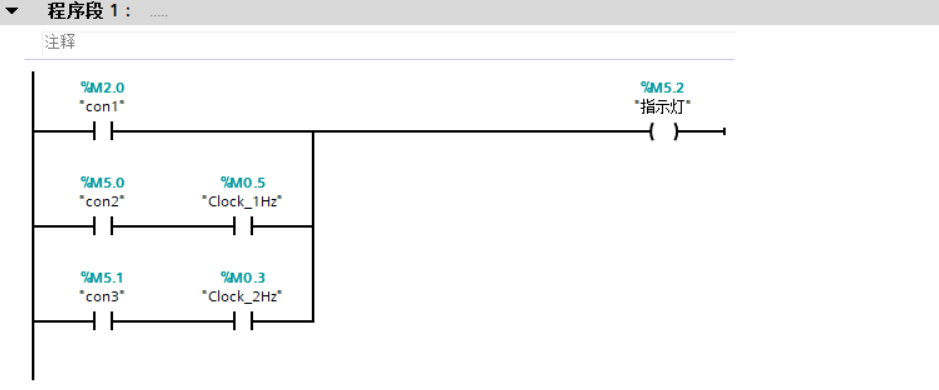
\includegraphics[width=.8\textwidth]{figure/程序段1.png} 
    \caption{程序段1} % caption是图片的标题
    % \label{img} % 此处的label相当于一个图片的专属标志,目的是方便上下文的引用
\end{figure}

\paragraph{程序段2}~{}

程序段2为SCL程序段,在此处定义了对于判断给定方程$ax^2 + bx + c = 0$解的情况的具体逻辑,以及对相应情况下指示灯闪烁方式的设置。首先根据$a$的值是否为零,将给定方程分类为一元二次方程或一元一次方程,且当$a= 0,\ b = 0$时,方程无解,此时为错误输入。当方程为一元二次方程时,对应的解有两个(两个实数解或一对共轭复数解),此时指示灯应以1s为周期闪烁;当方程为一元一次方程时,有一个解,此时指示灯应常亮;当输入参数错误导致方程无解时,指示灯应以0.5s为周期闪烁。此外,在各种情况下求得的方程的解都会在HMI界面中显示出来。
\begin{figure}[H]
    \centering % 居中 
    % 图片文件的相对路径
    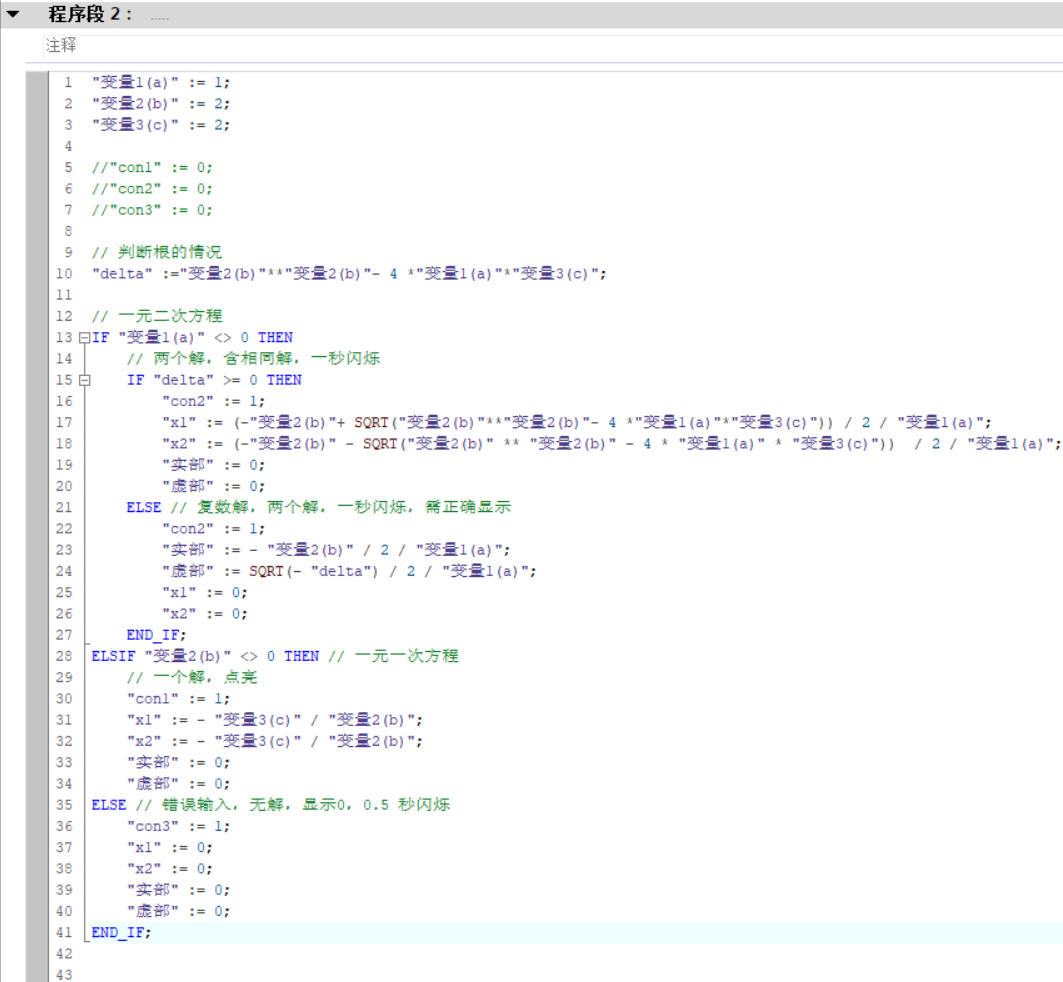
\includegraphics[width=.8\textwidth]{figure/程序段2.png} 
    \caption{程序段2} % caption是图片的标题
    % \label{img} % 此处的label相当于一个图片的专属标志,目的是方便上下文的引用
\end{figure}

%%
\subsection{HMI界面设计}
下图所示为自行设计的HMI界面,可以显示程序运行过程中各参数和变量的值:
\begin{figure}[H]
    \centering % 居中 
    % 图片文件的相对路径
    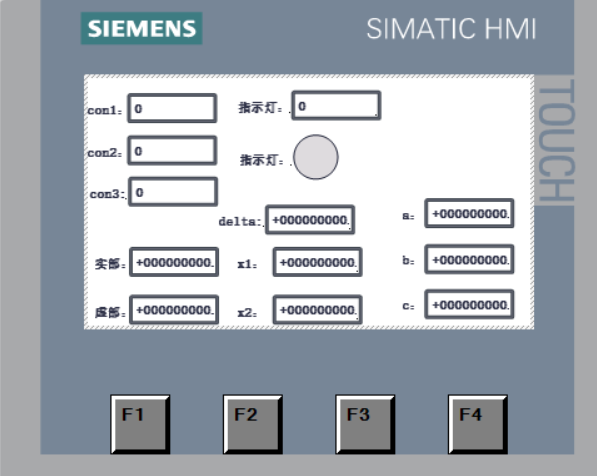
\includegraphics[width=.8\textwidth]{figure/HMI界面设计.png} 
    \caption{HMI界面设计} % caption是图片的标题
    % \label{img} % 此处的label相当于一个图片的专属标志,目的是方便上下文的引用
\end{figure}

\subsection{程序测试}
令$a = 1,\ b = 2,\ c = 1$,此时方程有两个解,对应$con2 = 1$:
\begin{figure}[H]
    \centering % 居中 
    % 图片文件的相对路径
    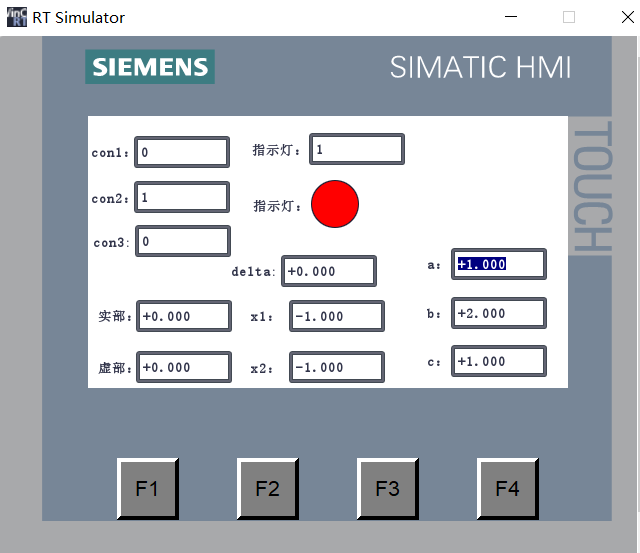
\includegraphics[width=.8\textwidth]{figure/相同解.png} 
    \caption{程序测试:两个解的情况} % caption是图片的标题
    % \label{img} % 此处的label相当于一个图片的专属标志,目的是方便上下文的引用
\end{figure}

令$a = 0,\ b = 2,\ c = 1$,此时方程有1个解,对应$con1 = 1$:
\begin{figure}[H]
    \centering % 居中 
    % 图片文件的相对路径
    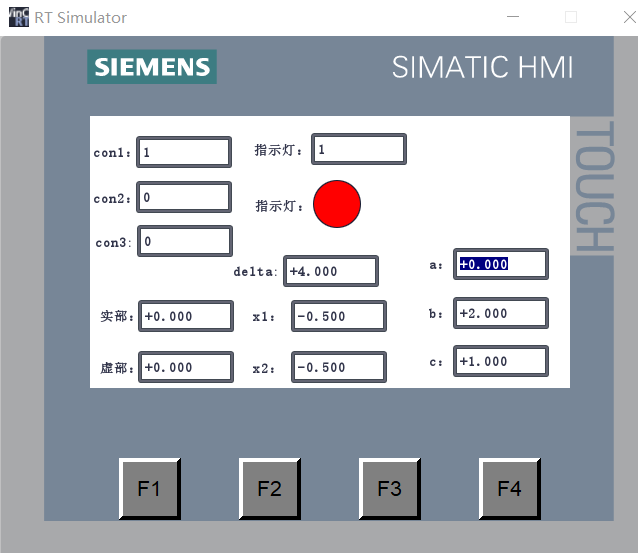
\includegraphics[width=.8\textwidth]{figure/一个解.png} 
    \caption{程序测试:1个解的情况} % caption是图片的标题
    % \label{img} % 此处的label相当于一个图片的专属标志,目的是方便上下文的引用
\end{figure}

令$a = 0,\ b = 0,\ c = 1$,此时方程无解,对应$con3 = 1$:
\begin{figure}[H]
    \centering % 居中 
    % 图片文件的相对路径
    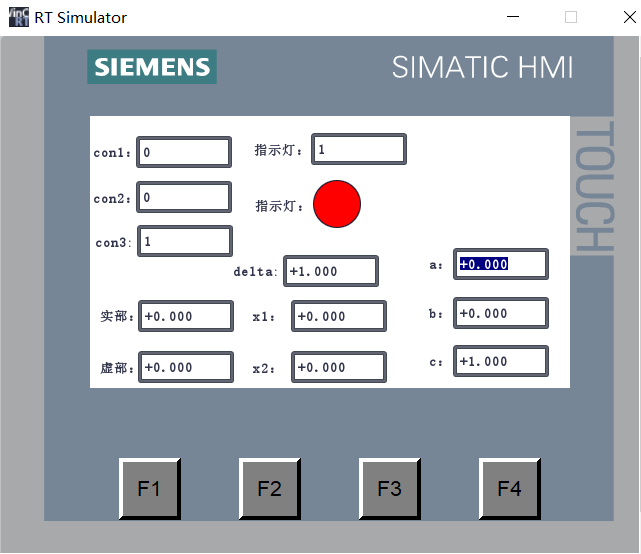
\includegraphics[width=.8\textwidth]{figure/无解.png} 
    \caption{程序测试:无解的情况} % caption是图片的标题
    % \label{img} % 此处的label相当于一个图片的专属标志,目的是方便上下文的引用
\end{figure}

\end{document}